\documentclass{article}
%Para imagenes
\usepackage{graphicx}
\usepackage{float}
\usepackage{enumitem} % Paquete para personalizar listas
\usepackage[margin=2cm]{geometry} % Ajusta todos los márgenes a 2 centímetros
\usepackage{indentfirst} % Este paquete fuerza la sangría del párrafo en la primera línea
\setlength{\parindent}{1cm} % Ajusta la sangría de los párrafos a 1 cm


\begin{document}
    \begin{titlepage}
        \centering
        {\bfseries\LARGE Universidad de Granada\par}
        \vspace{1cm}
        {\scshape\Large Facultad de Ingeniería Informática \par}
        \vspace{2cm}
        {\scshape\Huge Practica 2: Diseño adaptativo en Flutter \par}
        \begin{figure}[h]
                \centering
                
\includegraphics[width=0.6\textwidth]{logo_UGR.jpg}
                \label{fig:portada}
            \end{figure}
        {\itshape\Large DS: Grupo 1.7\par}
        \vfill
            {\Large  Emanuel Giraldo Herrera\par}
            {\Large  Thomas Lang \par}
            {\Large  Timur Sorokin \par}
            {\Large  Alejando Iborra Morán \par}
        \vfill
        {\Large (2023-2024) \par}
    \end{titlepage}

\tableofcontents

\newpage
\section{Introducción}
\subsection{Análisis del problema}
 
\subsection{Ingeniería inversa}


\newpage
\section{Desarrollo}
\subsection{Problemas encontrados}

\subsection{Widgets utilizados}

\subsection{Mejoras}



\newpage
\section{Ejecución}

\begin{figure}[h]
    \centering
    \vspace{5pt}
    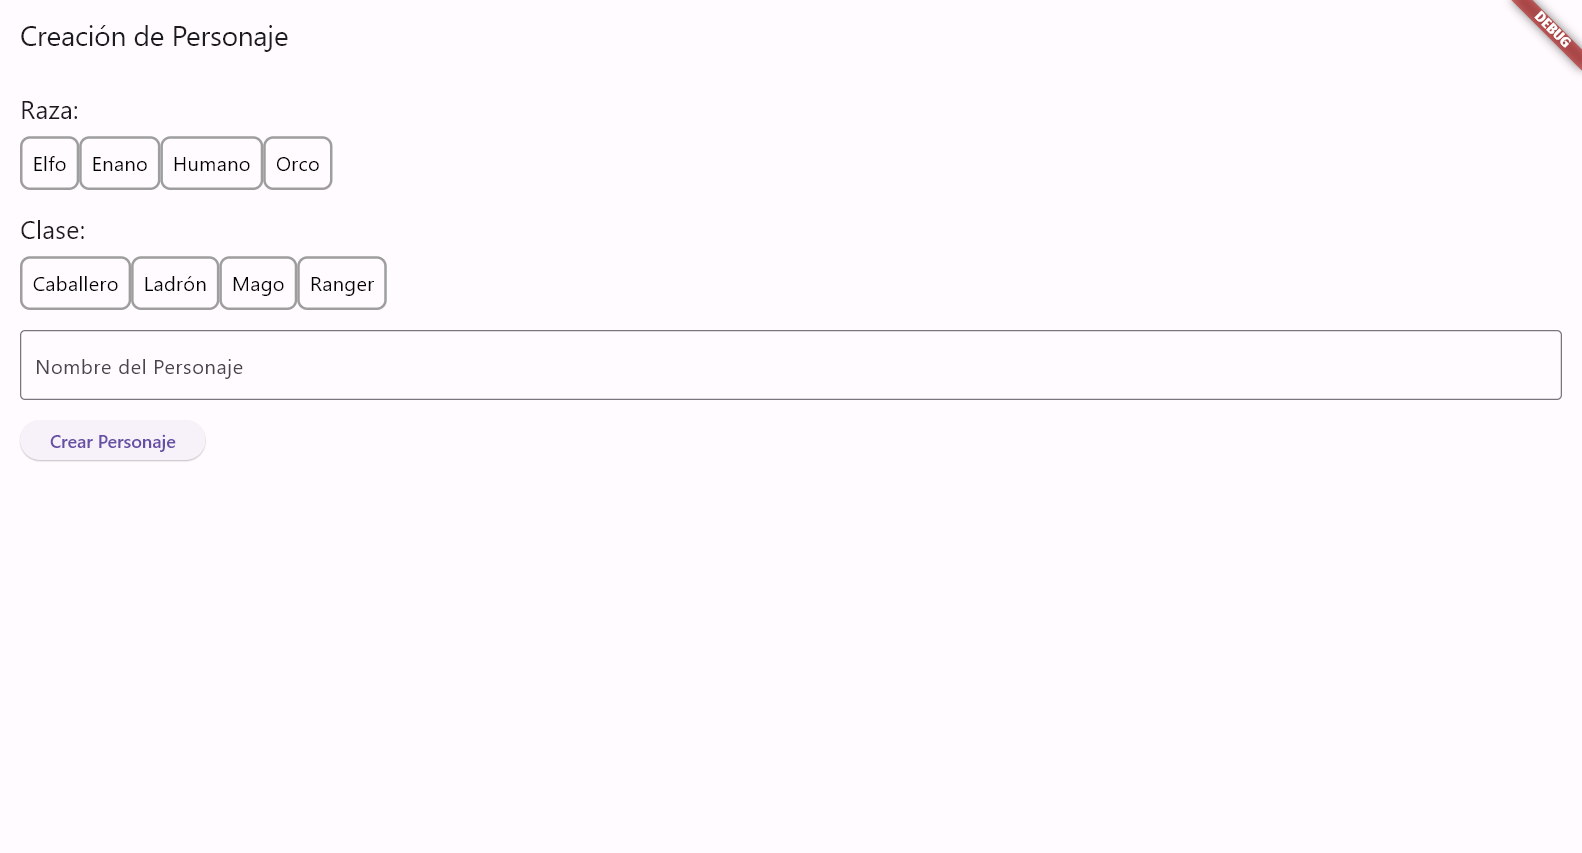
\includegraphics[width=0.9\textwidth]{Ejecucion_1.png}
    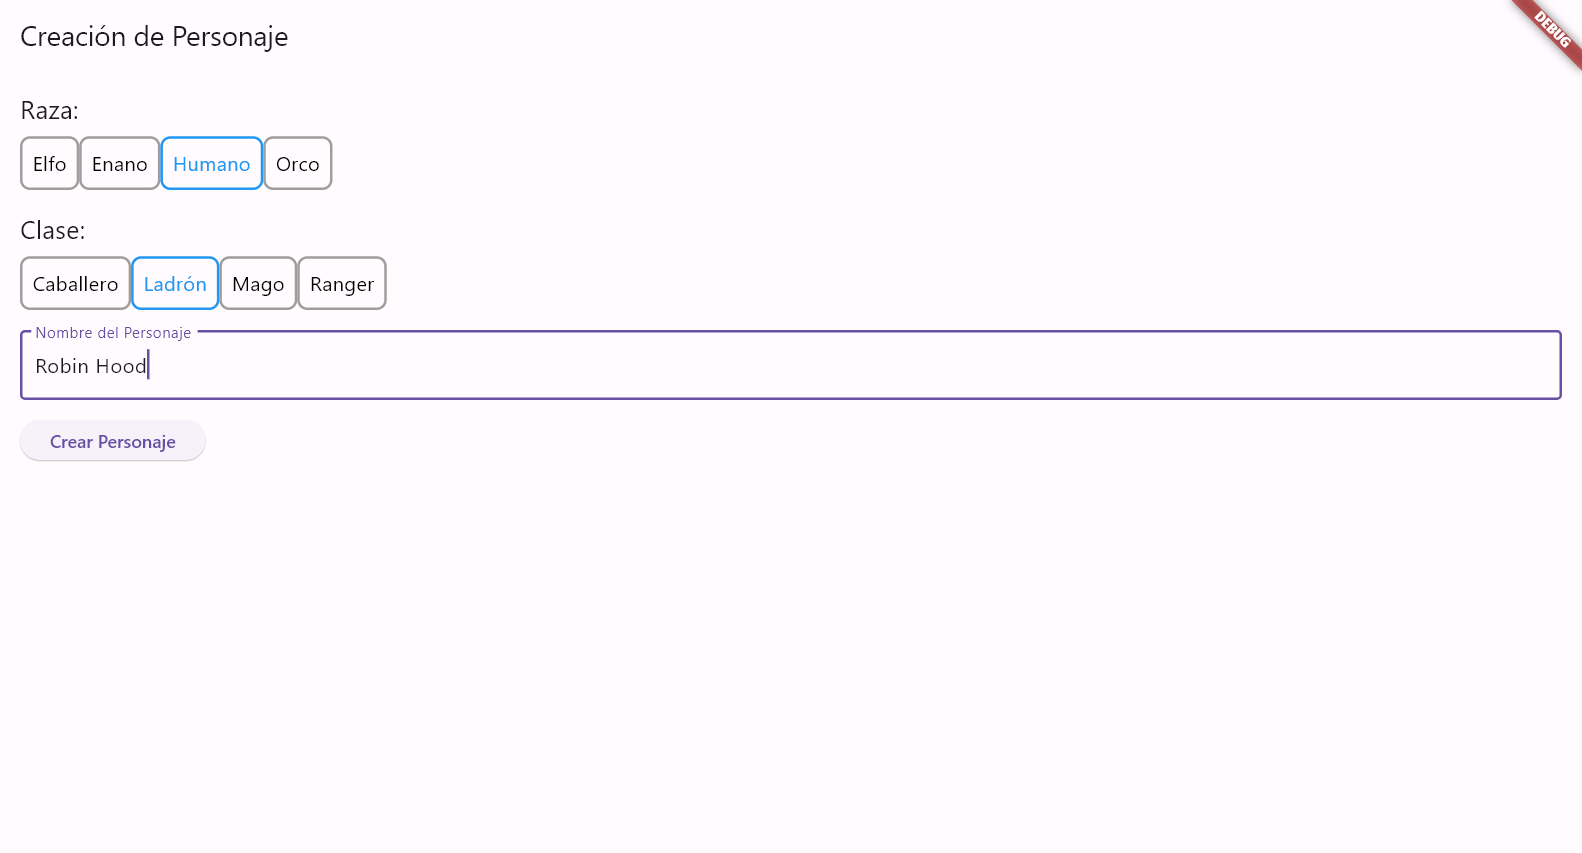
\includegraphics[width=0.9\textwidth]{Ejecucion_2.png}
    \caption{Pantalla de selección de personaje}
    \label{fig:ejecucion_1}
\end{figure}

\begin{figure}[h]
    \centering
    \vspace{5pt}
    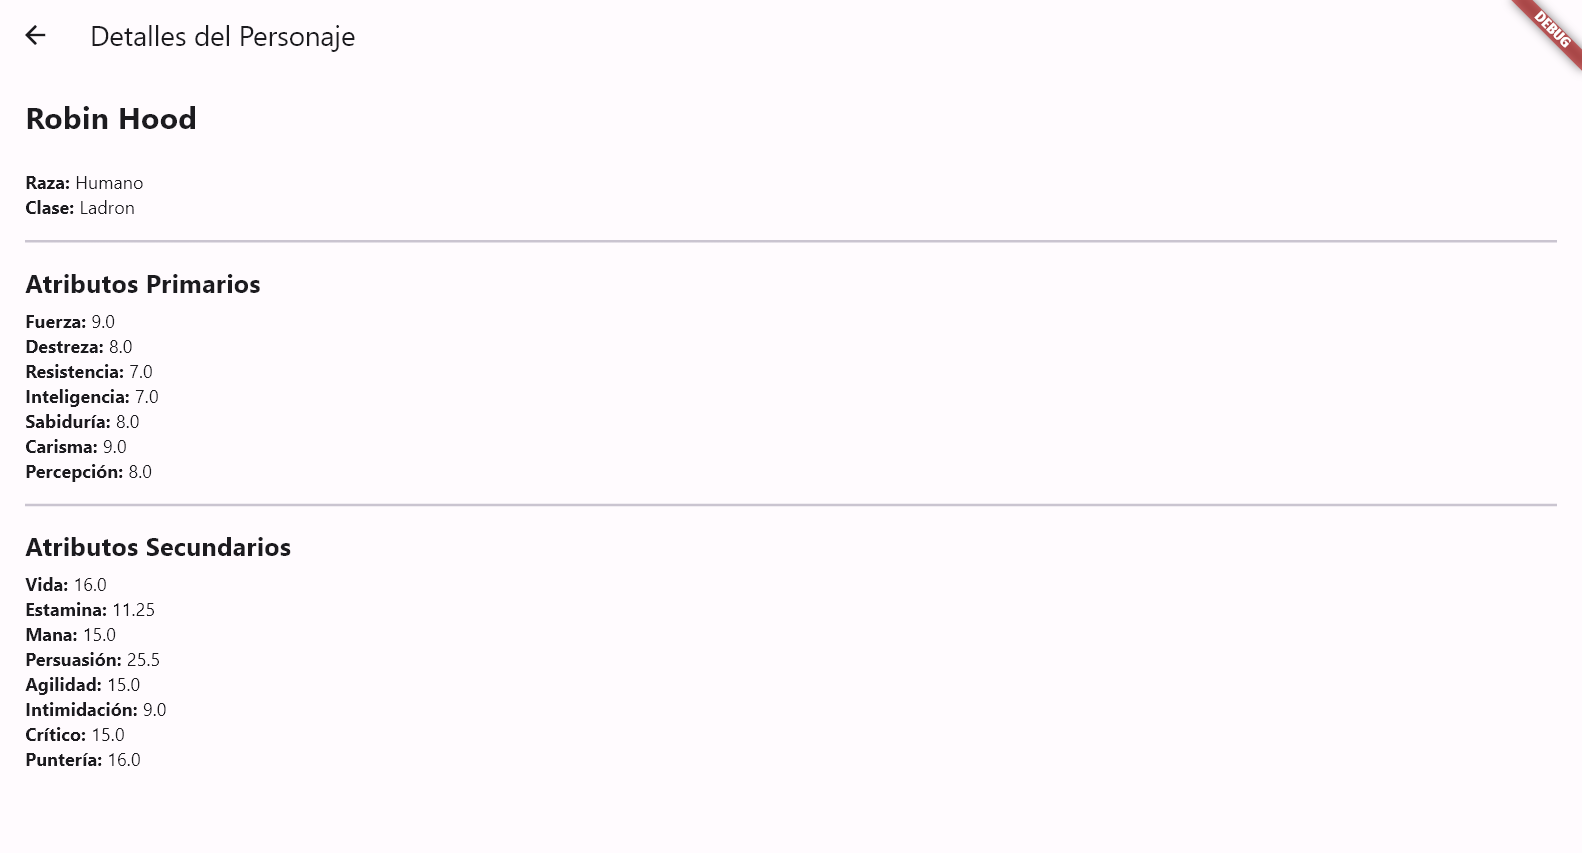
\includegraphics[width=0.9\textwidth]{Ejecucion_3.png}
    \caption{Pantalla de detalle del personaje}
    \label{fig:ejecucion_2}
\end{figure}



\end{document} 